\documentclass[11pt]{report}

\usepackage{epsf,amsmath,amsfonts}
\usepackage{graphicx}
\usepackage{listings}

\begin{document}

\title{Bit-For-Bit Reproducibility: \\
Requirements and Design}
\author{MPAS Development Team}

\maketitle
\tableofcontents

%-----------------------------------------------------------------------

\chapter{Summary}

This document is intended to describe options for creating bit-reproducible runs using the MPAS framework.

%-----------------------------------------------------------------------

\chapter{Requirements}

\section{Requirement: Bit Reproducibility}
Date last modified: 07/13/12
Contributors: (Michael Duda, Doug Jacobsen)

The only requirement for this project is to create an infrastructure that provides bit-reproducible runs using MPAS.

This requirement can be described as getting the exact (bit-for-bit) same result starting from the same initial conditions using an arbitrary number of blocks or processors.

In this case, bit-for-bit means you can subtract all fields from two output files and get identical zeros as a result.
%-----------------------------------------------------------------------

\chapter{Current Issues}

Within the current MPAS framework, there is an issue that causes non-bit-reproducible runs. This issue is caused by the unstructured ordering of elements such as edges and vertices. All elements within a single block are ordered based on halos rather than global ID index.

Within a processor, elements are stored with 0-halo elements first, followed by 1-halo elements, and 2-halo elements, etc. This ordering is then converted into a local ID ordering, with increasing local index however this creates random global ID ordering.

When computing certain operators, such as divergence, currently a loop over edges is used. Given a specific edge a flux is computed and the contribution is added to the neighboring cells that share an edge. Because of the local storage of edges, the contributions are added to a given cell in essentially random order when compared to other blocks/processors. This random accumulation of contributions causes non-bit-reproducible data for quantities such as divergence.

This issue can be seen in the following figure.
\begin{figure}[H!]
	\centering
	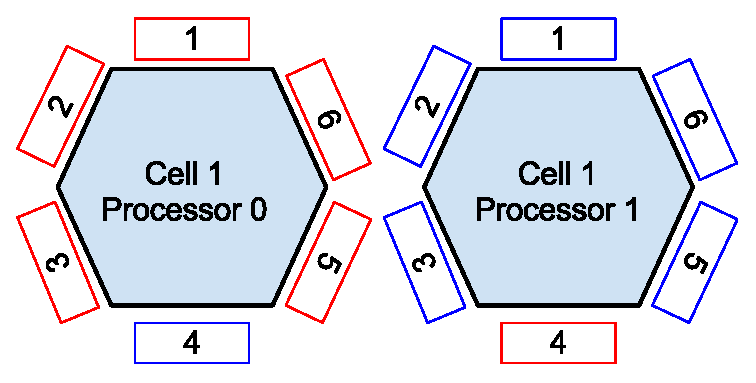
\includegraphics[scale=0.75]{Hexagons-NonBR.eps}
	\caption{The hexagon on the left is on by processor 0, while the hexagon on
	the right is the same hexagon on processor 1. Numbers indicate global edge
ID, while red boxed numbers indicate they belong in that processors 0 halo and
blue indicates they are in that processors 1 halo. Sums over edges happen on 0
halo edges before 1 halo edges.}
\end{figure}

\chapter{Design and Implementation}

\section{Option 1: Permutation Array}
Date last modified: 07/13/12
Contributors: (Michael Duda, Doug Jacobsen)

The first potential option for creating bit-reproducible simulations is to create a permutation array. This permutation array gives the index to edges/vertices in increasing global ID order which allows contributions to be accumulated in the correct order. This ordering is less efficient than the current ordering because all arrays based on edges/vertices are now accessed in random order as opposed to contiguously in memory.

This ordering could be turned on using either a compile or run-time flag. In order to ease development with this issue, it might be beneficial to provide a mpas\_edge\_index routine, and similar for the other elements. This routine would return either the globally ordered edge ID, or the locally ordered edge ID depending on compile-time/run-time flags. Loops over edges would now look like the following.

Also, to be able to preserve results, all loops now have to be performed over nEdges and nVertices as opposed to nEdgesSolve and similar. The nEdgesSolve arrays have no meaning when the permutation arrays are used and because of this is would be beneficial to overwrite all of these arrays with nEdges and similar to prevent issues related to not computing on a 0 halo.

\begin{lstlisting}[language=fortran,escapechar=@,frame=single]
do i = 1, nEdges
	iEdge = mpas_edge_index(i)
	... work on iEdge ...
end do
\end{lstlisting}

\section{Option 2: Re-index all arrays}
The second option might provide better performance but it has similar drawbacks to Option 1 in that loops now have to be over all elements as opposed to subsets of elements.

To accomplish this task, the permutation arrays could be computed as in option 1, and then before re-indexing from global id to local id all arrays can be permuted using this permutation array. Exchange lists will have to be permuted as well in order to have halo updates work the way they are supposed to. Permuting exchange lists should be as easy as re-indexing the srcList for sendLists, the destList for recvLists, and both the srcList and destList for copyLists.

This might provide better performance because now the increasing global ID is the same as increasing local ID, but loops cannot be restricted to owned elements anymore.

One potential down side is that I/O now requires a copy from the unordered element array to a list of owned elements, which requires a mask to be stored that now masks 0 halo edges and non 0 halo edges to allow easy copying.

%-----------------------------------------------------------------------

\chapter{Testing}
Date last modified: 07/13/12 
Contributors: (Michael Duda, Doug Jacobsen)

In order to test, the same configuration can be run on two different sets of blocks (1 block vs. 2 blocks) and all fields can be differenced (or the RMS can be taken). If the differences or RMS give identical zeros then testing is successful.

\chapter{Appendix}
\section{Array Limit Concerns}
One issue with the possible fixes for bit-reproducibility is that portions of arrays (the 0-halo for instance) can no longer be iterated over. The whole array needs to be iterated over because some of the 0-halo elements might exist beyond what the previous limits were.

In order to circumvent this issue a simple fix is proposed. This fix includes the addition of a new set of variables at the framework level. The table below shows what variables would be equal to under different run conditions in order to provide a straightforward change for bit reproducibility.

\begin{tabular}{| c | c | c | c |}
	\hline
					 & nEdges & nEdgesSolve & nEdgesOwned \\
	\hline
    bit-reproducible & nEdges & nEdges & nEdgesOwned \\
	\hline
not bit-reproducible & nEdges & nEdgesOwned & nEdgesOwned \\
	\hline
\end{tabular}

\section{I/O Layer Concerns in Option 2}
Within the proposed option 2 above, an issue is described where the I/O layer needs to be changed. This happens because the arrays are no longer stored with the first nEdgesOwned (using the terminology from the previous section) before any of the halo cells. Because of this storage difference, all owned elements need to be extracted and packed into their own array which can now be written to an output or restart file. The required changes could happen in the routine called MPAS\_writeStream within mpas\_io\_streams.F.

Currently, the code writes out temporary arrays with the required data in them. As an example, a 1d integer field is copied into a temporary array, and the temporary array is written to output. The following pseudocode shows an example of how the new code could look.

\begin{lstlisting}[language=fortran,escapechar=@]
#ifdef MPAS_BIT_REPRODUCIBLE
  copyElementIndex = 0
  do i = 1, totalElements
    if(ownedMask(i) == 1) then
	  copyElementIndex = copyElementIndex + 1
      int1d_temp(copyElementIndex) = outputField % array(i)
	end if
  end do
#else
  int1d_temp(:) = field_cursor % int1dField % array(:)
#endif
write_out(int1d_temp)
\end{lstlisting}

\section{Example of mpas\_get\_edge\_index function}

\begin{lstlisting}[language=fortran,escapechar=@]
integer function mpas_get_edge_index(grid, index)
  type (grid_type), intent(in) :: grid
  integer, intent(in) :: index

#ifdef MPAS_BIT_REPRODUCIBLE
  mpas_get_edge_index = grid % edgePermutationArray % array(index)
#else
  mpas_get_edge_index = index
#endif

  return
end function mpas_get_edge_index
\end{lstlisting}

%-----------------------------------------------------------------------

\end{document}
